\section{Rule-based modeling}

In the proposed model the compartments are Susceptible ($S$), Infectious ($I$), Recovered and Dead ($D$). Individuals either live in area one ($a_1$) or area two ($a_2$). They are non-vaccinated ($v_0$), vaccinated with vaccine one $(v_1)$ or vaccinated with vaccine two ($v_2$). Since we are dealing with two virus variants, the wild type $w$ and the mutant $m$, we account for this by introducing the feature $c_j$ with $j \in \{w,m\}$ that indicates the type of virus we are referring to. For infectious individuals we can distinguish between symptomatic $s_y$ and asymptomatic cases $s_n$.
 
We use the set notation of \cite{Waites.2021} to address certain subsets of the population. $\set()$ means all individuals. $\set(x_u)$ denotes all individuals from compartment $u \in \{S, I, R, D \}$, $\set(a_l)$ denotes all individuals from area $l \in \{1,2\}$, $\set(v_i)$ are all individuals with vaccination status $k \in \{0,1,2\}$, where zero indicates non-vaccinated, and $\set(c_j)$ are all individuals that currently have or had an infection with virus $j \in \{w,m\}$. With this notation we can pick desired subsets of the population by combining the appropriate features. All individuals from area one that are infected with the wild type are addressed by $\set(x_I, c_m)$. If we only want the unvaccinated individuals of them we use $\set(x_I, c_m, v_0)$. The usual set operators, like $\cup$. Using these operators allows us to address even more specific subsets like the set of all vaccinated individuals $\set(v_1) \cup \set(v_2)$. The set $\set()$ is defined as the whole population. The cardinalty $|\cdot|$ is used to addres the respective number of individuals in a set, e.g. $|\set(x_S, a_1)|$ equals the number of all susceptible individuals in area one.\\

In more specific cases it might be more comprehensive to replace the index numbers by meaningful abbreviations.

\subsection{Model}

\textbf{Assumptions so far:} 
\begin{itemize}
    \item distinction between symptomatic and asymptomatic infected cases only at recovered
    \item mutant can be more infectious but has same mortality. Additional parameter?
    \item no vaccination during infection \href{https://www.cdc.gov/vaccines/covid-19/info-by-product/clinical-considerations.html}{see here} (US Center for Disease Control)
    \item no births and other deaths
    \item no reinfection
\end{itemize}
\vspace{0.5cm}

\begin{itemize}
\item time dependence of parameters
\item cross-border with individuals being in the other country
\item rate of going somewhere must not be the same as people coming in (modify b function)
\item minimize over dead people or integrate of infected
\end{itemize}

\subsection{Transition Rates}

\subsubsection*{Vaccination}
For $j \in \{1,2\}$, $l \in \{1,2\}$
\begin{align*}
\set(x_S, v_0, a_l) &\xrightarrow{\nu_{j,l}(\cdot)} \set(x_S, v_j, a_l) \notag \\
\set(x_R, v_0, c_w, a_l) &\xrightarrow{\nu_{j,l}(\cdot)} \set(x_R, v_j, c_w, a_l)
\end{align*}
How to determine the vaccination rate? We denote the number of vaccinations of type $v_j$ available at time $t$ in country $l$ by $W_{j,l}(t)$ and the total number number of vaccine $j$ by $W_j(t) = W_{j,A}(t) + W_{j,B}(t)$. We assume that all doses of vaccines are immediately vaccinated. Thus, it must hold that 
\begin{align*}
W_{j,A}(t) &= \nu_{j, A} \cdot \left( |\set(x_S, v_0, a_A)| + |\set(x_R, v_0, a_A, c_w)| + |\set(x_R, v_0, a_A, c_m)| \right) \notag \\
W_{j,B}(t) &= \nu_{j, B} \cdot \left( |\set(x_S, v_0, a_B)| + |\set(x_R, v_0, a_B, c_w)| + |\set(x_R, v_0, a_B, c_m)| \right). 
\end{align*}
Which is to say that the total number of vaccines $j$ at $t$ must equal the number of individuals vaccinated with $j$ at $t$. Let $f_{j,A}(t)$ be the fraction of vaccine $j$ that is allocated to country $A$. We can write $W_{j,A}(t) = f_{j,A}(t) W_j(t)$ and $W_{j,B}(t) = \left[1 - f_{j,A}(t)\right] W_j(t)$. Combining both yields for country $A$ and $B$
\begin{align*}
\nu_{j,A} &= \frac{ f_{j,A}(t) W_{j}(t)}{|\set(x_S, v_0, a_A)| + |\set(x_R, v_0, a_A, c_w)| + |\set(x_R, v_0, a_A, c_m)|} \notag \\
\nu_{j,B} &= \frac{\left[1 - f_{j,A}(t)\right]  W_{j}(t)}{|\set(x_S, v_0, a_B)| + |\set(x_R, v_0, a_B, c_w)| + |\set(x_R, v_0, a_B, c_m)|}.
\end{align*}
To decide on the vaccination rates we therefore need to specify the trajectory of the fraction $f_{j,A}(t)$. Find appropriate function $g: \R^ \to [0,1]$. Let $y \in \R^b_+$ be the vector containing the number of individuals of the relevant compartments to consider and $z \in \R^b$ be parameters.  
\begin{itemize}
	\item logistic function $g(x \cdot z) = \frac{1}{1 + \exp(-y \cdot z)}$

\end{itemize}

  
\subsubsection*{Susceptible to Infectious}
To facilitate notation, we distinguish between individuals that are alive and those that are dead. We exclude all dead individuals by using prime notation to only address all living individuals, e.g. $\set'(a_l) =  \set(x_S, a_l) \cup \set(x_I, a_l) \cup \set(x_R, a_l)$. We define $N_l(t) = |\set'(a_l) |$ as the number of living individuals in area $l$ at time $t$. For specifying the transition rates we need to specify the probabilities that two individuals of a certain type meet. We do so by using the relative frequencies and adjust for cross-area meetings. The probability of an individual $i \in \set()$ to be in a particular subset is approximated by the relative frequencies. For example, the (time dependent) probability that a randomly drawn living individual is from area $l$ is $\prob\left(i \in \set'(a_l) \right) = \frac{N_l(t)}{N_1(t) + N_2(t)}$. To compute the probability that an individual is susceptible, conditioned that it is from area $l$, we can use Bayes' formula 
\begin{align}
\prob\left( i \in \set(x_S) |  i \in \set'(a_l) \right)= \frac{\prob\left(i \in  \set(x_S, a_l) \right)}{\prob\left(i \in \set'(a_l)\right)} = \frac{|\set(x_S, a_l)|}{|\set'(a_l)|} = \frac{|\set(x_S, a_l)|}{N_l(t)}.
\end{align}
We are interested in how many individuals are on average infected by an infected individual. To facilitate notation we assume that the infected individual lives in area one and is infected with the wild type $w$. The average number of infected individuals is a composition of the infection rate that is dependent on the virus type, the average number of contacts per infected individual and unit of time and the share of susceptible individuals that can be infected. We start with the baseline case of two unvaccinated individuals and first define the transition for susceptible individuals from area two.\\ 
Let $i_1 \in \set(x_I, v_0, c_w, a_1)$ and $i_2 \in \set()$.  We fix the location, vaccination status and compartment of individual one and allow individual two to potentially be from both areas and every compartment. We need to define $\prob(i_2 \in \set(x_S, v_0 ,a_2)|i_1 \in \set(x_I, v_0,c_w, a_1))$, the probability that the individual that can be infected is susceptible, unvaccinated and from area two given that individual one is infected with the wild type, unvaccinated and from area one. We assume that only the area has an influence on the probability of meeting an individual. The problem facilitates to finding $\prob(i_2 \in \set(x_S, v_0 ,a_2)|i_1 \in \set(a_1))$ or equivalently $\prob(i_2 \in \set(x_S, v_0) \wedge i_2 \in \set(a_2) | i_1 \in \set(a_1))$. Using Bayes' formula we can rewrite this as
\begin{align*}
\prob(i_2 \in \set(x_S, v_0) \wedge i_2 \in \set(a_2) | i_1 \in \set(a_1)) &= \prob(i_2 \in \set(a_2) | i_1 \in \set(a_1) )  \notag \\
& \quad \cdot \prob(i_2 \in \set(x_S, v_0) | i_1 \in \set(a_1), i_2 \in \set(a_2) ) \notag \\
&= \prob(i_2 \in \set(a_2) | i_1 \in \set(a_1) )  \notag \\
& \quad \cdot \prob(i_2 \in \set(x_S, v_0))
\end{align*} 
We first specify the probability $\prob(i_2 \in \set(a_2) | i_1 \in \set(a_1) )$, which is to say, the probability that $i_2$ is from area two. We cannot use the relative frequency of the number of individuals $\frac{N_{2}(t)}{N_1(t) + N_2(t)}$ as probability since this would not take into account that individuals meet more often within one region. We therefore add a penalty term $b\left(\text{d}(a_1, a_2) \right)$ that accounts for the distance between the areas
\begin{align*}
\prob(i_2 \in \set(a_2) | i_1 \in \set(a_1) ) = \frac{N_{2}(t)}{N_1(t) + N_2(t)} \cdot b\left(\text{d}(a_1, a_2) \right).
\end{align*}
$b(y) \in [0,1], b\left(0\right) = 1$ and $\lim\limits_{y \to \infty} b\left(y\right) = 0$. \textit{idea for} $b(y)= \frac{1}{1 + b y}$. Analogously we define the probabilities of $\prob(i_1 \in \set(a_1) | i_2 \in \set(a_2) )$. Subsequently, we use short-hand notation to address the conditional location probabilities. Let $m_{u,v}$ be the $u$-th row and $v$-th column of the Matrix $\vect{M} \in \R^{2 \times 2}$.
\begin{align*}
\vect{M} &= \begin{pmatrix} 
\prob(i_1 \in \set(a_1) | i_1 \in \set(a_1) ) & \prob(i_1 \in \set(a_1) | i_2 \in \set(a_2) ) \\
\prob(i_2 \in \set(a_2) | i_1 \in \set(a_1) ) & \prob(i_2 \in \set(a_2) | i_2 \in \set(a_2) )
\end{pmatrix} \notag \\
&= \begin{pmatrix} 
1 - \frac{N_{2}(t)}{N_1(t) + N_2(t)} \cdot b\left(\text{d}(a_1, a_2) \right) & \frac{N_{1}(t)}{N_1(t) + N_2(t)} \cdot b\left(\text{d}(a_1, a_2) \right) \\
\frac{N_{2}(t)}{N_1(t) + N_2(t)} \cdot b\left(\text{d}(a_1, a_2) \right) & 1 - \frac{N_{1}(t)}{N_1(t) + N_2(t)} \cdot b\left(\text{d}(a_1, a_2) \right)
\end{pmatrix}
\end{align*}

The probability of individual two to be unvaccinated and susceptible, conditioned that it is from area two, is taken to be the relative frequency of unvaccinated, susceptible individuals from area two
\begin{align*}
\prob(i_2 \in \set(x_S, v_0)) = \frac{|\set(x_S, v_0, a_2)|}{N_2(t)}
\end{align*}
Combining both results yields
\begin{align*}
\prob(i_2 \in \set(x_S, v_0 ,a_2)|i_1 \in \set(x_I, v_0,c_w, a_1)) = m_{2,1} \cdot \frac{|\set(x_S, v_0, a_2)|}{N_2(t)}
\end{align*}
Hence, $i_1$ meets on average $m_{2,1} c \frac{|\set(x_S, v_0, a_2)|}{N_2(t)}$ unvaccinated susceptible individuals from area two. At this meetings, $\alpha$ individuals become infected. This probability changes if we condition on the mutant. $i_1$ infects on average $\alpha m_{2,1} c \frac{|\set(x_S, v_0, a_2)|}{N_2(t)} $ individuals. This is done by $|\set(x_I, v_0, a_1)|$ individuals from area one and therefore we get the transitions $\alpha  m_{2,1} c \frac{|\set(x_S, v_0, a_2)|}{N_2(t)} |\set(x_I, v_0, a_1)|$
Using rule-based notation we write this as 
\begin{align*}
\set(x_{I},  v_0, c_w,a_1), \set(x_{S}, v_0, a_2) &\xrightarrow{ \frac{\alpha  m_{2,1} c}{N_2(t)} } \set(x_{I},v_0, c_w,a_1), \set(x_{I}, v_0, c_w, a_2)
\end{align*}
Same but for unvaccinated from same area (\textit{we ignore minus one})
\begin{align*}
\set(x_{I},  v_0, c_w,a_1), \set(x_{S}, v_0, a_1) &\xrightarrow{\frac{\alpha  m_{1,1} c}{N_1(t)}} \set(x_{I},  v_0, c_w,a_1), \set(x_{I},  v_0, c_w,a_1)
\end{align*}
The extension to the mutant and vaccinated individuals is straightforward by multiplying the probability that a meeting of an individual with the base virus type and a susceptible individual results in an infection. We assume that if the infected individual is vaccinated, this reduces the infection probability by the factor $1 -\gamma$ for $\gamma \in [0,1]$. For $k \in \{1,2\}$ and $l \in \{1,2\}$
\begin{align*}
\set(x_{I},  v_k, c_w, a_1), \set(x_{S}, v_0, a_l) &\xrightarrow{\frac{(1-\gamma) \alpha  m_{1,l} c}{N_l(t)}} \set(x_{I},  v_k, c_w,a_1), \set(x_{I},  v_0, c_w,a_l).
\end{align*}
We interpret $\gamma$ as degree of protection against spreading the virus after being vaccinated.

If the susceptible individual is vaccinated with vaccine $k \in \{1,2\}$ we assume that this reduces the infection probability for virus type $j \in \{w,m\}$ by the factor $1 - \delta_{j,k}$ for $\delta_{j,k} \in [0,1]$. For $k \in \{1,2 \}$ and $l \in \{1,2\}$
\begin{align*}
\set(x_{I},  v_0, c_w, a_1), \set(x_{S}, v_k, a_l) &\xrightarrow{\frac{(1-\delta_{w,k}) \alpha  m_{1,l} c}{N_l(t)}} \set(x_{I},  v_0, c_w, a_1), \set(x_{I},  v_k, c_w, a_l).
\end{align*}
We can interpret $\delta_{j,k}$ as degree of protection against virus type $j$ we gain from being vaccinated with vaccine $k$. In the extreme case where $\delta_{j,k} = 1$ vaccine $k$ gives a full protection against virus $j$ and no infections with virus $j$ are possible for individuals vaccinated with $k$. Analogously, $\delta_{j,k} = 0$ means that there is no additional protection at all.

We allow the mutant to be more or less infectious than the wild type by introducing the additional parameter $\eta \in \left(0, \frac{1}{\alpha}\right]$. $\eta > 1$ means that the mutant is more infectious than the wild type. \textit{maybe restrict to this case?} 
For $l \in \{1,2\}$
\begin{align*}
\set(x_{I},  v_0, c_m, a_1), \set(x_{S}, v_0, a_l) &\xrightarrow{\frac{ \eta \alpha  m_{1,l} c}{N_l(t)}} \set(x_{I},  v_0, c_m, a_1), \set(x_{I},  v_0, c_m, a_l).
\end{align*}
We can combine the factors for different infection probabilities. For example the transition from the infectious individuals from area one, infected with the mutant, and vaccinated with vaccine one and the susceptible individuals vaccinated with vaccine two is for $l \in \{1,2\}$
\begin{align*}
\set(x_{I},  v_1, c_m, a_1), \set(x_{S}, v_2, a_l) &\xrightarrow{\frac{ \eta \alpha (1-\delta_{m,2}) (1-\gamma)  m_{1,l} c}{N_l(t)}} \set(x_{I},  v_1, c_m, a_1), \set(x_{I},  v_2, c_m, a_l).
\end{align*}

\subsubsection*{Infectious to Recovered/Death}
non-vaccinated. For $l \in \{1,2\}$
\begin{align}
    \set(x_I,  v_0, c_w, a_l) &\xrightarrow{p \lambda} \set(x_D,  v_0, c_w, a_l) \notag \\
\set(x_I,  v_0, c_w, a_l) &\xrightarrow{(1-p) \lambda} \set(x_R,  v_0, c_w, a_l) \notag \\
\end{align}

vaccinated. For $k \in \{1,2\}$ and $l \in \{1,2\}$
\begin{align}
    \set(x_I,  v_k, c_w, a_l) &\xrightarrow{\omega_{k,w} p \lambda} \set(x_D,  v_k, c_w, a_l) \notag \\
\set(x_I,  v_k, c_w, a_l) &\xrightarrow{(1-\omega_{k,w}p) \lambda} \set(x_R,  v_k, c_w, a_l) \notag 
\end{align}


\subsection{Graphical model description}
On the next page you find a graphical representation of the model using tikz. I have omitted the second region and cross-border infections from the graph to increase readability.  

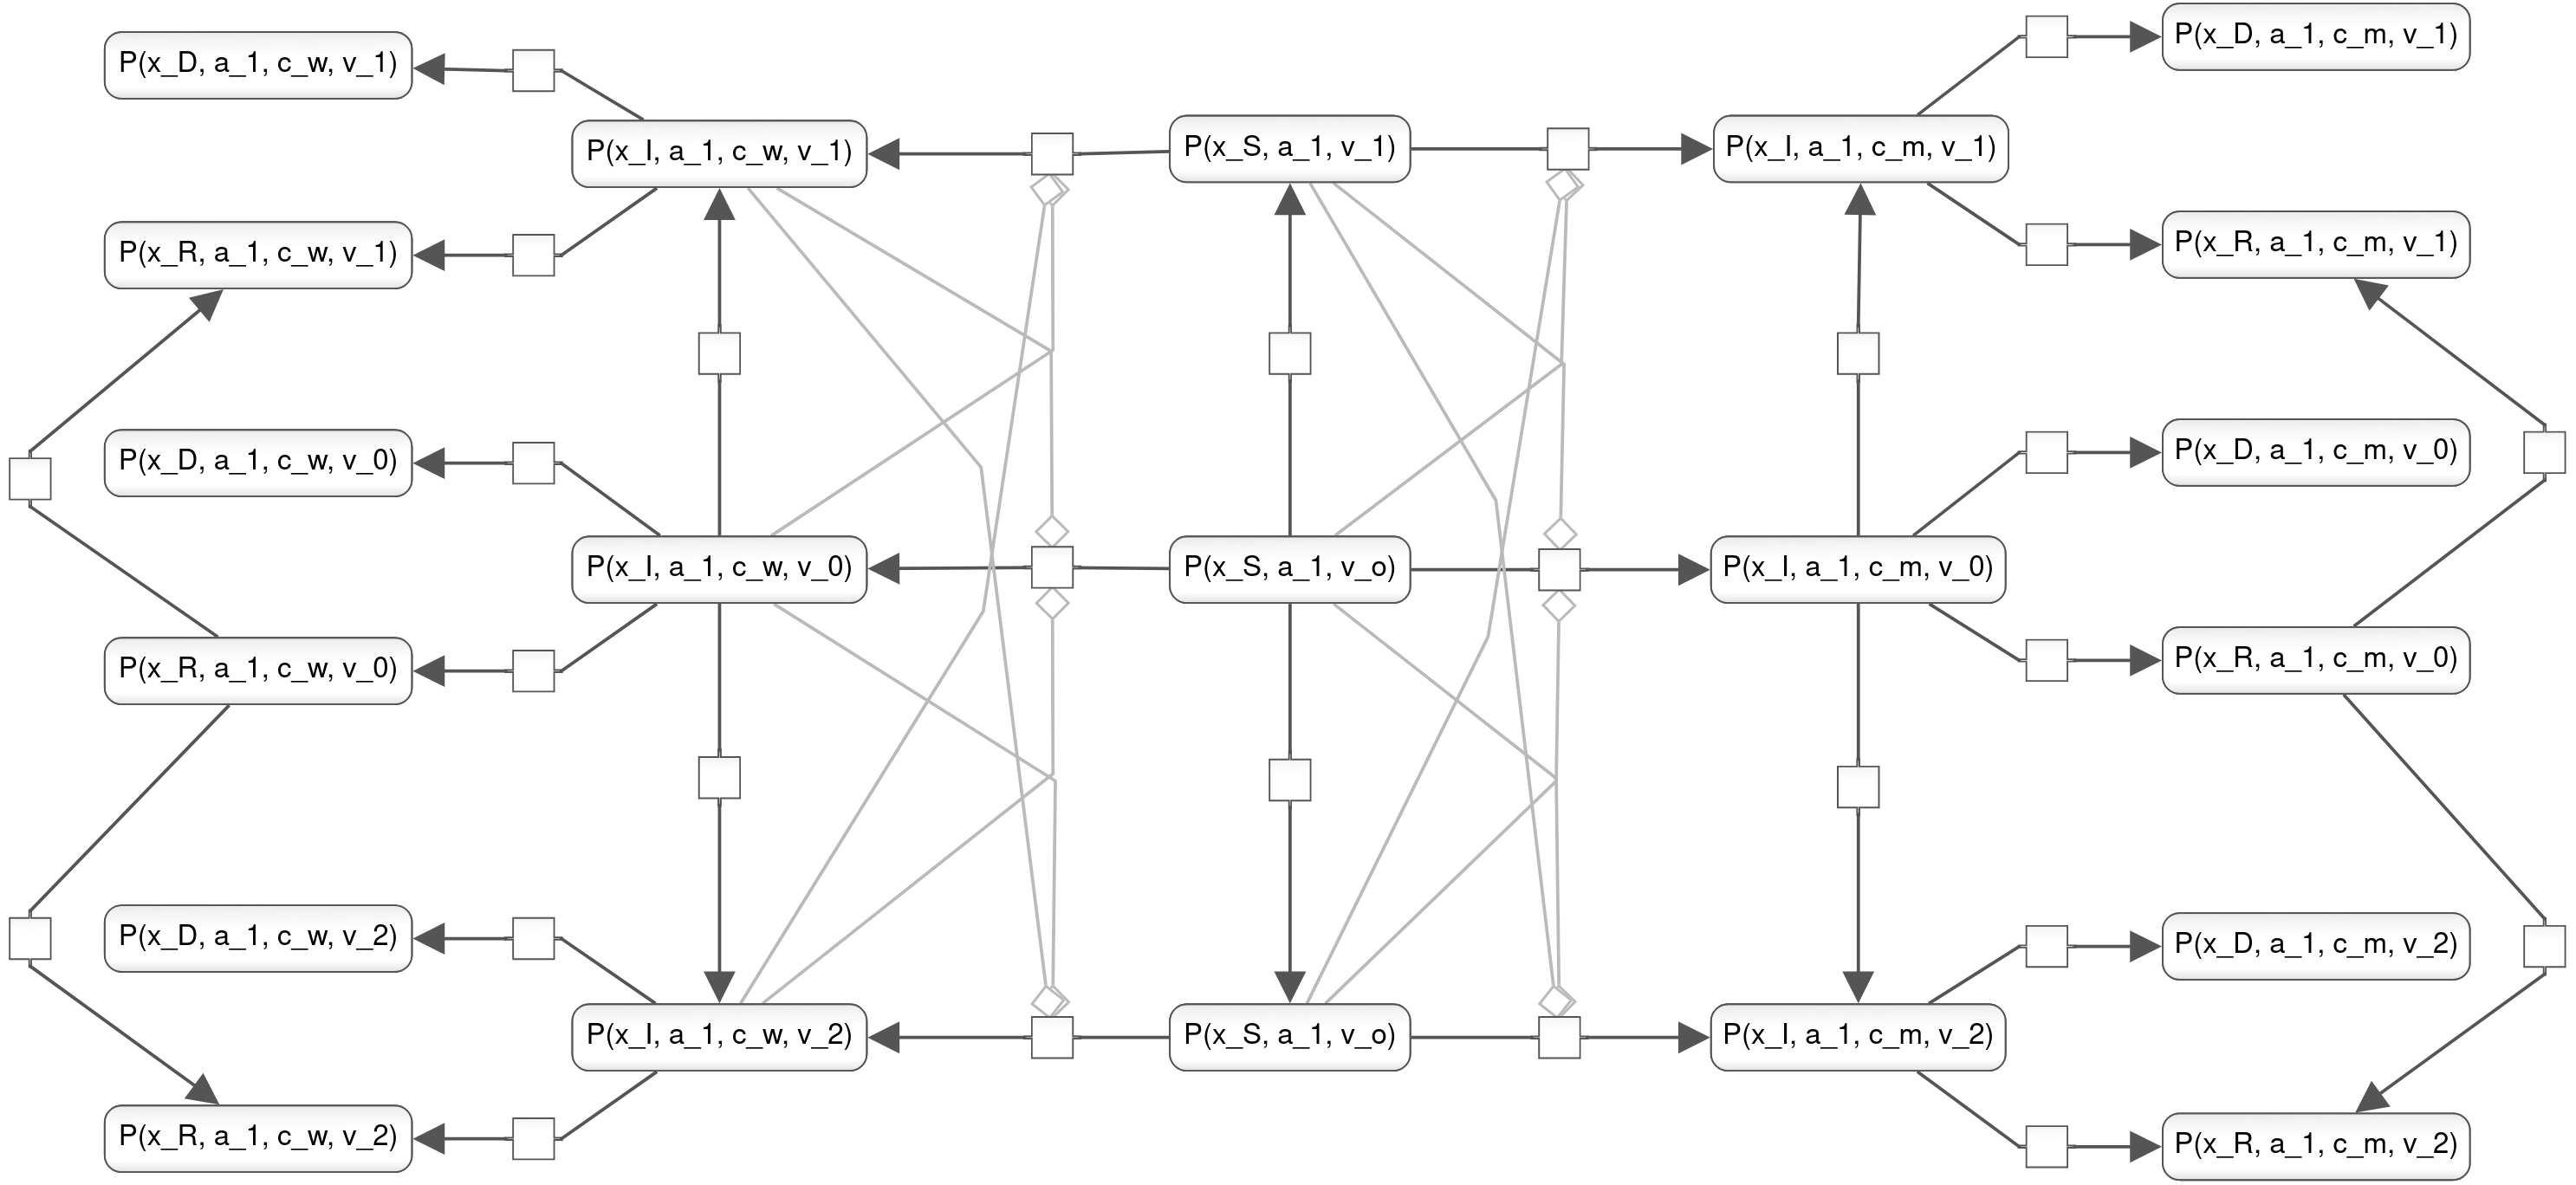
\includegraphics[scale=0.15]{images/vaccination.png}